% Course Exam Style
% By: Hamid Zarrabi-Zadeh
% Licenced Under GPL

\documentclass[11pt,a4paper]{article}

\usepackage{graphicx,comment,framed}
\usepackage{amsthm,amssymb,amsmath}
\usepackage{enumitem}
%\usepackage[colorlinks,linkcolor=blue,citecolor=blue]{hyperref}

\usepackage[localise=on, extrafootnotefeatures]{xepersian}
\usepackage[noend]{algpseudocode}


%--------------------- page settings ----------------------

\settextfont[Scale=1.1]{XB Niloofar}
\setdigitfont[Scale=1.1]{XB Niloofar}
%\defpersianfont\sayeh[Scale=1.1]{XB Kayhan Pook}
\addtolength{\textheight}{3.2cm}
\addtolength{\topmargin}{-24mm}
\addtolength{\textwidth}{3cm}
\addtolength{\oddsidemargin}{-1.5cm}

\renewcommand{\labelitemi}{$\small\bullet$}
\renewcommand{\arraystretch}{1.3}


%------------------------ Environments ------------------------------------

\newtheorem{قضیه}{قضیه}
\newtheorem{لم}{لم}
\newtheorem{مشاهده}{مشاهده}
\newtheorem{تعریف}{تعریف}


%-------------------------- Notations ------------------------------------

\newcommand{\IR}{\ensuremath{\mathbb{R}}} 
\newcommand{\IZ}{\ensuremath{\mathbb{Z}}} 
\newcommand{\IN}{\ensuremath{\mathbb{N}}} 
\newcommand{\IS}{\ensuremath{\mathbb{S}}} 
\newcommand{\IC}{\ensuremath{\mathbb{C}}} 
\newcommand{\IB}{\ensuremath{\mathbb{B}}} 

\newcommand{\bR}{\mathbb{R}}
\newcommand{\cB}{\mathcal{B}}
\newcommand{\cO}{\mathcal{O}}
\newcommand{\cG}{\mathcal{G}}
\newcommand{\rM}{\mathrm{M}}
\newcommand{\rC}{\mathrm{C}}
\newcommand{\rV}{\mathrm{V}}

\newcommand{\ceil}[1]{{\left\lceil{#1}\right\rceil}}
\newcommand{\floor}[1]{{\left\lfloor{#1}\right\rfloor}}
\newcommand{\prob}[1]{{\mbox{\tt Pr}[#1]}}
\newcommand{\set}[1]{{\{ #1 \}}}
\newcommand{\seq}[1]{{\left< #1 \right>}}
\newcommand{\provided}{\,|\,}
\newcommand{\poly}{\mbox{\rm poly}}
\newcommand{\polylog}{\mbox{\rm \scriptsize polylog}\,}
\newcommand{\divs}{\ | \ }
\newcommand{\congruent}[1]{\,\overset{#1}{\equiv}\,}

\newcommand{\lee}{\leqslant}
\newcommand{\gee}{\geqslant}
\renewcommand{\leq}{\lee}
\renewcommand{\le}{\lee}
\renewcommand{\geq}{\gee}
\renewcommand{\ge}{\gee}

\newcommand{\REM}[1]{}
\renewcommand{\حذف}{\REM}
\newcommand{\mrbox}[1]{\mbox{\lr{#1}}}

\newcommand{\لر}{\lr}


\newcounter{probcnt}
\newcommand{\مسئله}[1]{\stepcounter{probcnt}\bigskip\bigskip{
 	\large \bf مسئله‌ی \arabic{probcnt}$\mbox{\bf{.}}$ \ #1} \bigskip}

\newcommand{\fqed}[1]{\leavevmode\unskip\nobreak\quad\hspace*{\fill}{\ensuremath{#1}}}

\newenvironment{اثبات}
	{\begin{trivlist}\item[\hskip\labelsep{\em اثبات.}]}
	{\fqed{\square}\end{trivlist}}

\newenvironment{حل}
	{\begin{trivlist}\item[\hskip\labelsep{\bf حل.}]}
	{\fqed{\blacktriangleright}\end{trivlist}}

\ifdefined\hidesols
	\newsavebox{\trashcan} % uncomment the following line to hide solutions
	\renewenvironment{حل}{\begin{latin}\begin{lrbox}{\trashcan}}{\end{lrbox}\end{latin}}
\fi


%------------------------- Header -----------------------------

\newcommand{\سربرگ}[3]{
\parindent=0em

\rightline{
\makebox[5em][c]{
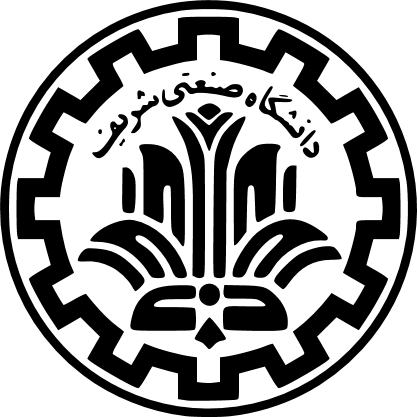
\includegraphics[height=1.5cm]{../commons/sharif.png}
}}
\vspace{-.2em}
{\scriptsize\bf دانشکده‌ی مهندسی کامپیوتر}
\hfill {\small
مدرس:  آبام-بهرامی \  
}\\[-5em]
\leftline{\hfill\large\bf 
ساختمان‌داده‌ها و الگوریتم‌ها
}\\[.2em]
\leftline{\hfill\bf 
نیم‌سال اول ۰۲-۰۳
}\\[1.4em]
\hrule height .12em

\small
\vspace{1mm} 
نام و نام خانوادگی:
\hfill #2 %[2mm]
%شماره‌ی دانش‌جویی:
%\hfill  زمان: #3
%\vspace{1.5mm} 
\hrule height .1em

\vspace{-5.7em} 
\hfill {\large #1} \hfill
\vspace*{4em}
}

\newcommand{\نام‌دانش‌جو}[2]{
\begin{framed}
نام دانش‌جو: #1\hfill شماره‌ی دانش‌جویی: #2
\end{framed}
}

\pagestyle{empty} 



\شروع{نوشتار}


\سربرگ{آزمون پایان‌ترم}{۲۴ دی ۱۴۰۲}{۱۵۰ دقیقه}
\medskip

\مسئله{میزبانی جام‌ ملت‌های آسیا }[۱۳ نمره]

قرار است میزبان جام ملت‌های آسیای دوره‌ی بعد بزودی مشخص شود.  لیست نامزدها مشخص است و کنفدراسیون فوتبال آسیا (ای‌اف‌سی) بررسی‌های  لازم خود را از کشورهای نامزد  انجام داده است. باتوجه به بررسی‌های انجام شده، درحال حاضر مشخص است اگر ای‌اف‌سی بخواهد بین دو   کشور نامزد $A$ و $B$ یکی را انتخاب کند کدام کشور را انتخاب خواهد کرد. سیستم انتخاب میزبان توسط ای‌اف‌سی بدین‌شکل است. در هر مرحله از بین نامزدهای باقی‌مانده، دو  نامزد را بطور کاملا تصادفی انتخاب می‌کند و نامزدی که رای ای‌اف‌سی با او نیست را حذف می‌کند. با فرض آنکه نظر ای‌اف‌سی را در مورد هر دو کشور نامزد می‌دانیم، می‌خواهیم کشورهایی که شانس کسب میزبانی را دارند را پیدا کنیم.  برای این کار یک گراف جهت‌دار $n$ راسی  می‌سازیم که $n$ تعداد کشورهای نامزد است و هر راس متناظر با یک کشور نامزد است. برای هر دو راس $A$ و $B$ یک یال بین آن‌ها می‌گذاریم و جهت یال را به سمت کشوری می‌گذاریم که نظر ای‌اف‌سی با آن کشور است. 
\شروع{شمارش}
\فقره نشان دهید کشور $A$ شانس میزبانی دارد اگر و فقط اگر از همه‌ی رئوس به راس $A$ مسیر وجود داشته باشد. (۶ نمره)
\فقره الگوریتمی با زمان اجرای $\Theta(n^2)$ ارائه دهید که تمام کشورهایی که شانس میزبانی را دارند را پیدا کند. دقت کنید که تعداد یال‌های گراف از  $\Theta(n^2)$ است. (۷ نمره)
 \پایان{شمارش}
 \مسئله{وارسی خطی}[۱۲ نمره]
 
 فرض کنید از آدرس‌دهی باز و وارسی خطی برای درهم‌سازی استفاده شده  و تابع درهم سازی $i^2$ به پیمانه ۷ است. بعد از دریافت همه اعداد
  $\{0,\dots, 6\}$ می‌دانیم نحوه‌ی قرار گیری اعداد در جدول درهم‌ساز به صورت زیر است:
 
 $$A[0,..,6] = 0,6, 4, 3, 1,5,2$$
 
 به ازای چند جایگشت ورودی وضعیت جدول درهم‌ساز به شکل بالا خواهد بود.
 
 
\مسئله{ظرفیت درهم‌سازی} [۲۰ نمره]

$ \mathcal{H} $
یک خانواده‌ی درهم‌ساز $ 2 $-فراگیر است (\lr{2-Universal Hash Family}) اگر برای هر دو عدد متمایز $ x_1 $ و $ x_2 $ داشته باشیم
$ Pr[h(x_1) = h(x_2)]  \leq \frac{1}{n}$
که $ h $ به صورت تصادفی یکنواخت از $ \mathcal{H} $ انتخاب می‌شود.
حال فرض کنید
$ \mathcal{H} = \{h_1, h_2\} $
که

$ h_1, h_2: \{0, \dots, n\} \rightarrow \{0, \dots, m\} $ 
می‌باشند.
\شروع{شمارش}[label=(\alph*)]
\فقره اگر $ m = 1 $ باشد، حداکثر مقدار عدد $ n $ برای آنکه این خانواده ۲-فراگیر باشد چند است؟ (۱۲ نمره)
\فقره حداکثر مقدار عدد $ n $ بر حسب $ m $ برای آنکه این خانواده ۲-فراگیر باشد چند است؟ (۸ نمره) 
\پایان{شمارش}

\newpage
\مسئله{مسیر صحیح}[۲۰ نمره]

در این سوال قصد داریم مسئله‌ی کوتاه‌ترین مسیر را برای گراف‌هایی که وزن یال‌هایشان صحیح است بررسی کنیم. به این صورت که وزن یال‌های گراف از مجموعه‌ی
$ \{1, \dots, I\} $
انتخاب شده است.
\شروع{شمارش}[label=(\alph*)]
\فقره نشان دهید حداکثر فاصله‌ی میان دو رأس یا بی‌نهایت ($ \infty $) است و یا حدکثر $ I(n-1) $. (۳ نمره)
\فقره در صورت استفاده از الگوریتم دایکسترا، ثابت کنید فاصله‌ی رأس‌های اضافه شده به درخت کوتاه‌ترین مسیر تا مبدأ در هر مرحله (خروجی \texttt{Extract-Min}) غیر نزولی است. (۵ نمره)
\فقره الگوریتم دایکسترا را طوری تغییر دهید که کوتاه‌ترین مسیر را در زمان 
$ \mathcal{O}(IV+E) $
محاسبه کند. (۱۲ نمره)
%\فقره فرض کنید اگر وزن یال‌های گراف داده شده را در نظر نگیریم، طولانی‌ترین مسیری که الگوریتم \lr{BFS} از رأس $ s $ می‌یابد حداکثر $ m $ یال داشته باشد. آیا می‌توان تغییری در الگوریتم \lr{Bellman-Ford-Moore} ایجاد کرد که حداکثر پس $ m+1 $ مرحله الگوریتم پایان پذیرد؟ (دقت کنید $ m $ در ابتدا مشخص نیست)
\پایان{شمارش}

\مسئله{مجزا بازی}[۱۵ نمره]
\شروع{شمارش}[label=(\alph*)]
\فقره داده‌ساختار جنگل مجموعه‌های مجزا با استفاده از \lr{{Union By Rank}} و \lr{{Path Compression}} و عناصر اولیه‌ی 
$ \{1\}, \{2\}, \dots, \{10\} $
داده شده است. پس از انجام اعمال زیر وضعیت این داده‌ساختار را با رسم شکل نشان دهید (هنگام استفاده از \lr{{Union By Rank}} در صورت تساوی عدد کوچکتر را ریشه قرار دهید). (۵ نمره)
\begin{LTR}
\texttt{union(1, 2), union(3, 4), union(5, 6), union(7, 8), union(1, 4),\\
union(6, 7), union(4, 5), find(1), union(9, 8), union(10, 3), find(3)
}
\end{LTR}
\فقره فرض کنید مجموعه‌های مجزا را به کمک  \lr{{Union By Rank}} و \textbf{بدون} \lr{{Path Compression}}  پیاده‌سازی کردیم. دنباله‌ای از $ m $ عمل 
\texttt{union} و \texttt{find}
بر روی $ ‌n $ عنصر ارائه دهید که زمان اجرای آن‌ها
$ \Omega(m\log{n}) $
باشد. (۱۰ نمره)
\پایان{شمارش}

\مسئله{تک درخت‌}[۲۰ نمره]

گراف هم‌بند و بدون جهت $  G = (V, E) $ و راس $ v \in V $ از آن داده شده است. می‌دانیم \lr{BFS} و \lr{DFS}ی با شروع از رأس $ v $ وجود دارد که درخت‌های ریشه‌دار \lr{BFS} و \lr{DFS} یکسان شده است. درستی گزاره‌های زیر را رد یا اثبات کنید.
\شروع{شمارش}[label=(\alph*)]
\فقره حداکثر تعداد رئوس $ G $ برابر ۳ است. (۱۰ نمره)
\فقره $ G $ یک درخت است. (۱۰ نمره)

%\فقره $ G $ دو بخشی است.
\پایان{شمارش}
\پایان{نوشتار}
